\chapter{\ifenglish Background Knowledge and Theory\else ทฤษฎีที่เกี่ยวข้อง\fi}

การทําโครงงานให้มีความสําเร็จเเละมีความสมบูรณ์ จําเป็นต้องศึกษาค้นคว้าทฤษฎีที่เกี่ยวข้อง ซึ่งเนื้อหาใน
บทนี้จะเกี่ยวกับการอธิบายถึงสิ่งที่เกี่ยวข้องกับโครงงาน เพื่อให้ผู้อ่านเข้าใจเนื้อหาในบทถัดไปได้ง่ายมากขึ้น
โดยจะเเบ่งเนื้อหาหลักออกมาได้ดังนี้

\section{ทฤษฎีการเขียนโปรแกรมเชิงวัตถุ หรือ object-oriented programming (OOP)}
การเขียนโปรแกรมเชิงวัตถุ(object-oriented programming: OOP) ก็คือการเขียนโปรแกรมเชิงวัตถุ ซึ่ง
เป็นแนวคิดในการพัฒนาซอฟแวร์ที่เป็นที่ยอมรับ เนื่องจากซอฟแวร์ที่ถูกพัฒนาและใช้กันอยู่นั้น นับวันมีแต่
จะซับซ้อนมากยิ่งขึ้น ถ้าหากไม่จัดการกับโค้ดให้ดีพอก็อาจจะทําให้การพัฒนาล่าช้าหรือไม่สําเร็จได้OOP จึง
ออกแบบมาให้โค้ดที่เราเขียนมีแบบแผนที่เหมาะสมพร้อมใช้ในการพัฒนาที่ซับซ้อนได้ โดยมองสิ่งต่างๆ ใน
ระบบเป็นวัตถุ (objects) ชิ้นหนึ่งที่มีหน้าที่และความหมายในตัว โดยวัตถุนั้นๆ ก็มีคุณสมบัติ(attributes)
และพฤติกรรม (methods หรือ behaviors) หรือการกระทําของมัน เป็นการมองบนพื้นฐานความเป็นจริง
มากขึ้น นอกจากนี้ oop\cite{oop} ยังสามารถนําไปไปประยุกต์ในเชิง softaware design ซึ่งเราได้นําเอาเเนวคิด oop มาประยุกต์ใช้เพื่อออกเเบบ Data model เเละ Database ของระบบ

\section{HTML (Hypertext Markup Language)}
HTML\cite{html} ย่อมาจาก Hypertext Markup Language เป็นภาษาที่ใช้ในการแสดงผลในเว็บบราวเซอร์บนอินเตอร์เน็ต สามารถแสดงข้อมูลตัวอักษร ภาพ, เสียง และไฟล์ในรูปแบบอื่นๆ โดยโครงสร้างหลักของ HTML
ก็จะเริ่มด้วย <html> และจบด้วย </html> เสมอ เเละยังมีtags ต่างๆ ที่หลากหลายให้ใช้งานตามความ
ต้องการ ซึ่งชุดคําสั่งที่ใช้จะแยกเป็น 2 ส่วน ได้แก่
\begin{enumerate}
  \item head คําสั่งที่อยู่ในส่วนนี้จะใช้อธิบายรายละเอียดเกี่ยวกับ web page จะแสดงผลอย่างไรที่ web
  page โดยตรง
  \item body คําสั่งที่อยู่ในส่วนนี้จะใช้ในการจัดรูปแบบตัวอักษร จัดหน้า ใส่รูปภาพ ซึ่งตัวอักษร ในส่วนนี้จะ
  ต่างจากข้างบนอย่างไร โดยตรงเช่น ข้อความ, รูปภาพ, เสียง, วีดิโอ หรือไฟล์ต่างๆ  
\end{enumerate}

\section{Typescript}
TypeScript\cite{type} คือ Super Set ของ JavaScript ที่จุดเด่นคือถูกพัฒนาให้มี strongly typed ทําให้ต้องระบุ type ของตัวแปรให้ชัดเจนก่อนจึงจะสามารถเรียกใช้งานและรันโค้ดต่อไปได้ ซึ่งจะช่วยให้โปรเเกรมมีความเเน่นหนาขึ้น ผู้พัฒนาสามารถพัฒนาโปรเจคได้อย่างมีประสิทธิภาพ ทำความเข้าใจได้ง่าย และสามารถป้องกันความผิดพลาดหรือช่องโหว่ของ JavaScript’s error เมื่อทำการ compile 

\section{JSON (JavaScript Object Notation)}
JSON\cite{json} เป็นฟอร์แมตสำหรับการแลกเปลี่ยนข้อมูลที่เป็นที่นิยมในปัจจุบัน เนื่องจากว่าฟอร์แมตมีขนาดเล็กและโครงสร้างที่ไม่ซับซ้อน 
ทำให้ในการเก็บข้อมูลนั้นสั้นกระชับ ไม่ต้องใช้พื้นที่ในการเก็บโครงสร้างของข้อมูลมากเกินความจำเป็น และนำไปใช้งานได้เร็ว โดยเฉพาะเมื่อนำไปใช้ใน 
JavaScript จะสามารถแปลงเป็น JavaScript Object และใช้งานได้ทันที โดยประเภทของข้อมูลที่ JSON เก็บมีดังนี้
\begin{enumerate}
  \item string - เป็นประเภทข้อมูลแบบข้อความที่ประกอบไปด้วยหลายตัวอักษรโดยจะใช้เครื่องหมาย double-quote (“ ”) เป็นตัวบ่งบอก
  \item number - เป็นประเภทข้อมูลที่เป็นตัวเลข
  \item object (JSON object) - เป็นประเภทข้อมูลที่ประกอบด้วยสองส่วนได้แก่ key และ value ซึ่งจะใช้ colon (:) ในการแบ่งระหว่างทั้งสองตัว และสามารถเก็บ key และ value ได้หลายตัวใน object เดียวกัน โดยจะใช้ comma (,) เพื่อแบ่งแต่ละคู่ เช่น 
  { key: value1 , key: value2 , key: value3}
  \item array - เป็นประเภทข้อมูลที่มีหน้าตาคล้ายตารางหรือ list คือจะมีข้อมูลที่เรียงต่อกันอยู่ใน array นั้น โดยจะใช้ square bracket ([ ]) เป็นตัวบ่งบอกและใช้ comma (,) เป็นตัวแบ่งแต่ละค่าใน array ตัวอย่างเช่น [ value1, value2, value3 ]
  \item boolean - เป็นประเภทข้อมูลที่เป็น true หรือ false ซึ่งข้อมูลชนิดนี้จะแสดงได้ค่าใดค่าหนึ่งเท่านั้นไม่สามารถแสดงพร้อมกันทั้งสองค่าได้
  \item null - เป็นประเภทข้อมูลที่บอกถึงค่าว่าง
\end{enumerate}


\section{React}
React\cite{react} เป็น JavaScript library ที่ใช้สำหรับสร้าง user interface (UI) ที่ให้ผู้พัฒนาสามารถเขียนโค้ดในการสร้างส่วนต่างๆที่มีความซับซ้อนแบ่งเป็นส่วนเล็กๆที่เรียกว่า component ออกจากกันได้ ซึ่งแต่ละส่วนสามารถแยกการทำงานออกจากกันได้อย่างอิสระ และทำให้สามารถนำชิ้นส่วน component เหล่านั้นไปใช้ซ้ำได้อีก โดยภาษาที่รองรับในการเขียนคือ JSX (JavaScript syntax extension) และ TSX (TypeScript syntax extension) 
ซึ่งเป็นการเขียนที่คล้ายกับ JavaScript และ HTML แต่สิ่งที่ต่างออกไปคือสามารถเขียน component ลงไปในไฟล์ JavaScript ได้เลย และ React จะใช้ JSX ในการแสดงผลเว็บไซค์ต่อไป และนอกจากนี้ยังมีคอนเซปต์หลักของ React ที่ช่วยให้เขียนโค้ดได้ง่ายและไวขึ้น ได้แก่
\begin{enumerate}
  \item Component - คือส่วนต่างๆที่แสดงผลบนหน้าเว็บไซค์ เช่น navbar, button และ content เป็นต้น 
  หรือสรุปได้ว่าทุกส่วนที่แสดงผลบนหน้าเว็บไซค์ล้วนถูกเรียกว่า component ทั้งสิ้น
  \item State - คือข้อมูลที่อยู่ใน component แต่ละส่วน ซึ่งใน React จะมีเครื่องมือที่ช่วยในการเปลี่ยน state 
  เพื่อให้ผู้พัฒนาเขียนโค้ดง่ายขึ้นเรียกว่า React hook
  \item Props - คือข้อมูลที่ถูกส่งต่อจาก component ชั้นบนไปยังชั้นล่าง หรือ parents component ไปยัง child component 
  โดยค่าที่ส่งไปนั้นสามารถเป็นได้ทั้ง ค่าคงที่, ตัวแปร, ฟังก์ชัน และ component ด้วยกันเอง 
\end{enumerate}

\section{NodeJS}
Node.js\cite{node} เป็น open-source และ cross-platform JavaScript runtime environment 
ที่ได้รับความนิยมอย่างสูง Node.js ทำให้เราใช้ JavaScript ในฝั่ง Server ได้ 
โดยหน้าที่อยู่ที่ฝั่ง Backend ทำตัวเป็น Web Server จากเดิมที่เคยอยู่ฝั่ง Frontend ทำหน้าที่ร่วมกันกับ html
ซึ่ง Node.js สามารถรันได้บน platform ที่หลากหลาย
จุดเด่นที่สุดของ Node.js คือมันทำงานแบบ asynchronous Node.js จะมี APIs ที่เราสามารถใช้สำหรับทำงานกับระบบปฏิบัติการ 
เช่น การรับค่าและการแสดงผล การอ่านเขียนไฟล์ และการทำงานกับเน็ตเวิร์ก เป็นต้น เเละ มี Node package manager เป็นตัวจัดการ package เสริมต่างๆมากมายที่
เราสามารถติดตั้งเพื่อใช้งานเพิ่มเติม


\section{ExpressJS}
Express.js\cite{express} หรือ Express นั้นเป็นเว็บเฟรมเวิร์กจาก NPM (Node Package Manager) ที่ใช้สําหรับ
พัฒนาเว็บแอพพลิเคชันหรือเว็บไซต์บน Node.js ที่ทํางานที่ฝั่งของ Backend ตัวของเฟรมเวิร์คนั้นถูกพัฒนา
มาจากโมดูล HTTP ซึ่งเป็นโมดูลของ Node.js เอง แต่เราใช้มันเพื่อทําให้การพัฒนาเว็บแอพพลิเคชันบน
Node.js ทําได้ง่ายขึ้น และ Express.js มีคุณสมบัติที่โดดเด่นคือ
\begin{enumerate}
  \item มีการจัดการ routing ที่เข้าใจง่าย 
  \item ฟังก์ชันช่วยสําหรับ HTTP\cite{http}
  \item ทํางานได้รวดเร็วและมีประสิทธิภาพ
  \item เป็น framework ที่นิยม มี community ให้ค้นคว้า เเละเเก้ปัญหาที่ครบถ้วน
  \item สามารถทํางานร่วมกับ GraphQL ได้อย่างมีประสิทธิภาพ ด้วย apollo-server-express
\end{enumerate}

\section{GraphQL}
GraphQL\cite{graphql} คือ ภาษาสําหรับการเข้าถึงข้อมูล (query language) เพื่อการใช้งาน API ของระบบและประมวลผลคําสั่งที่ฝั่ง server หรือที่เรียกว่า server-side runtime 
โดยใช้โครงสร้างข้อมูลที่เรากําหนดไว้ มีคุณสมบัติ ที่ใช้งาน เข้าใจง่าย ไม่ซับซ้อน และให้ผลลัพธ์ได้ตรงตามความต้องการของผู้ใช้งาน 
การใช้GraphQL สามารถจัดการเพียงแค่ข้อมูลที่เราต้องการใช้ออกมา ทําให้เราสามารถปรับเปลี่ยน (customize) รูปแบบ
องข้อมูลที่เราจะนําไปใช้ต่อได้ตามต้องการ ด้วยการสืบค้น (query) และเปลี่ยนแปลง (mutate) ข้อมูล
ซึ่งเป็นวิธีการหลัก ของ GraphQL โดยไม่ยุ่งยาก ส่งผลให้ข้อมูลที่ได้จากฐานข้อมูลมีประสิทธิภาพมากขึ้น
ผ่านหลักการคือ หลังจากเราส่ง request เพื่อไปดึงข้อมูลมาจาก API ผลลัพธ์ที่ได้จะถูกส่งกลับมาในรูปแบบ
ของ JSON (JavaScript Object Notation) ทําให้เราสามารถใช้ข้อมูลในรูปแบบที่เเตกต่างในสถานการณ์
ที่หลากหลายได้ เช่น บน web platform เราต้องการใช้ข้อมูลทั้งหมด ในขณะที่บน mobile platform พื้นที่
(space) จํากัด เราอาจจะต้องการใช้ข้อมูลเพียงบางส่วน ทําให้ในปั จจุบันถูกนําไปใช้งานอย่างแพร่หลายใน
หลายบริษัทชั้นนํา

\section{NoSQL}
ฐานข้อมูล NoSQL\cite{no} สร้างตามวัตถุประสงค์สําหรับโมเดลข้อมูลแบบเฉพาะเจาะจงและมีแบบแผนที่ยืดหยุ่น
เเละเป็นที่รู้จักกันดีในด้านความง่ายในการพัฒนา การทํางาน และประสิทธิภาพตามขนาดที่ต้องการ มีการ
ใช้โมเดลข้อมูลที่หลากหลายสําหรับการเข้าถึงและจัดการข้อมูล ฐานข้อมูลประเภทนี้ได้รับการปรับปรุงประสิทธิภาพสําหรับแอปพลิเคชันที่ต้องใช้ข้อมูลปริมาณมาก มีเวลาแฝงตํ่า ซึ่งเกิดขึ้นโดยการผ่อนปรนข้อจํากัด
ความสมํ่าเสมอข้อมูลของฐานข้อมูลอื่นๆ ฐานข้อมูล NoSQL เหมาะสมมากสําหรับแอปพลิเคชันสมัยใหม่
เช่น อุปกรณ์เคลื่อนที่ เว็บ และเกมที่จําเป็นต้องมีฐานข้อมูลที่ปรับขนาดได้ ประสิทธิภาพสูง และทํางานได้ดี
เยี่ยมเพื่อมอบประสบการณ์ผู้ใช้ที่ยอดเยี่ยม โดยมีคุณสมบัติที่เป็นจุดเด่น ดังนี้
\begin{enumerate}
  \item ความยืดหยุ่น: มีแบบแผนยืดหยุ่นที่ทําให้การพัฒนาเกิดขึ้นเร็วและทําซํ้าคําสั่งได้ดียิ่งขึ้นกว่าเดิม โมเดลข้อมูลที่ยืดหยุ่นทําให้ฐานข้อมูล NoSQL เหมาะสมที่สุดสําหรับข้อมูลแบบกึ่งมีโครงสร้างและไม่มี
  โครงสร้าง
  \item ความสามารถในการปรับขนาด: ปรับขนาดออกได้โดยใช้คลัสเตอร์แบบกระจายของฮาร์ดแวร์ แทน
  การปรับขนาดขึ้นโดยเพิ่มเซิร์ฟเวอร์ที่มีราคาแพงและมีประสิทธิภาพสูง ผู้ให้บริการระบบคลาวด์บาง
  เจ้าจัดการปฏิบัติการนี้อยู่เบื้องหลังในแบบบริการที่มีการจัดการเต็มรูปแบบ
  \item ประสิทธิภาพสูง: ฐานข้อมูล NoSQL ได้รับการปรับปรุงประสิทธิภาพสําหรับโมเดลข้อมูลบางโมเดล
  และเข้าถึงรูปแบบที่เปิดใช้งานประสิทธิภาพที่สูงกว่าการพยายามดําเนินการทํางานที่คล้ายกันด้วยฐาน
  ข้อมูลเชิงสัมพันธ์
  \item ทํางานได้ดีเยี่ยม: ฐานข้อมูล NoSQL มีAPI การทํางานและประเภทข้อมูลที่สร้างตามวัตถุประสงค์
  สําหรับโมเดลข้อมูลแต่ละโมเดลที่สอดคล้องกัน
\end{enumerate}

\section{MongoDB}
MongoDB\cite{mongo} เป็น Open-Source Document Database รูปแบบหนึ่ง ที่เป็นฐานข้อมูลแบบ NoSQL มีการ
จัดเก็บข้อมูลอยู่ในรูปแบบ BSON ที่มีความเร็ว เเละประสิทธิภาพสูง ซึ่งเหมาะสมอย่างมากในการจัดการข้อมูลที่มีจํานวน
มาก เพราะจุดเด่นอยู่ที่ความเร็วในการทํางานเป็นหลัก คิวรี่ข้อมูลได้เร็วขึ้น การทํางานในส่วนของ database จะลดลง แต่
จะไปเน้นการทํางานในส่วนของโปรแกรมที่พัฒนาขึ้นมาแทน เเละยังมีความยืดหยุ่นมากในการเก็บข้อมูล เนื่องจากสามารถจัดเก็บข้อมูลได้หลากหลาย 
เช่นการ input ข้อมูลรูปเเบบ ตารางที่มาจาก Database ที่เป็น SQL

\section{ทฤษฎีความตัดกันของสี}
ในการออกแบบหน้าตาของ web application เพื่อให้เกิดความสวยงามนั้น จําเป็นที่จะต้องคํานึงถึงการเลือก
ใช้สีให้มีความเหมาะสมต่อผู้ใช้งาน เพื่อไม่ให้สีนั้นเกิดความฉูดฉาดหรือเด่นชัดจนเกินไป รวมถึงไม่ให้สีดูกลมกลืนกันกับพื้นหลังมากเกินไปด้วยเช่นกัน จนเกิดความยากลําบากในการอ่าน ดังนั้น ผู้พัฒนาจึงใช้เว็บไซต์ชื่อ
WebAIM: contrast Checkerเพื่อเป็นตัวช่วยในการเทียบค่าความตัดกันของสีที่เลือกใช้


\section{การคํานวณเกรด}
การคํานวณเกรดเฉลี่ยจะใช้สูตรคํานวณต่อไปนี้
\begin{equation}\label{eq:grade}
  GPA = \frac{\sum_{i=1}^{n}{G_i}\cdot{P_i}}{\sum_{i=1}^{n}{P_i}}
\end{equation}
โดยที่
\noindent
  \begin{itemize}
    \item GPA คือเกรดเฉลี่ยโดยรวม
    \item $G_i$ คือเกรดที่ได้ในวิชาที่ $𝑖$
    \item $P_i$ คือหน่วยกิจที่ได้ในวิชาที่ $𝑖$ 
    \item $𝑛$ คือจํานวนวิชา
  \end{itemize}
\begin{figure}[h!]
  \begin{center}
    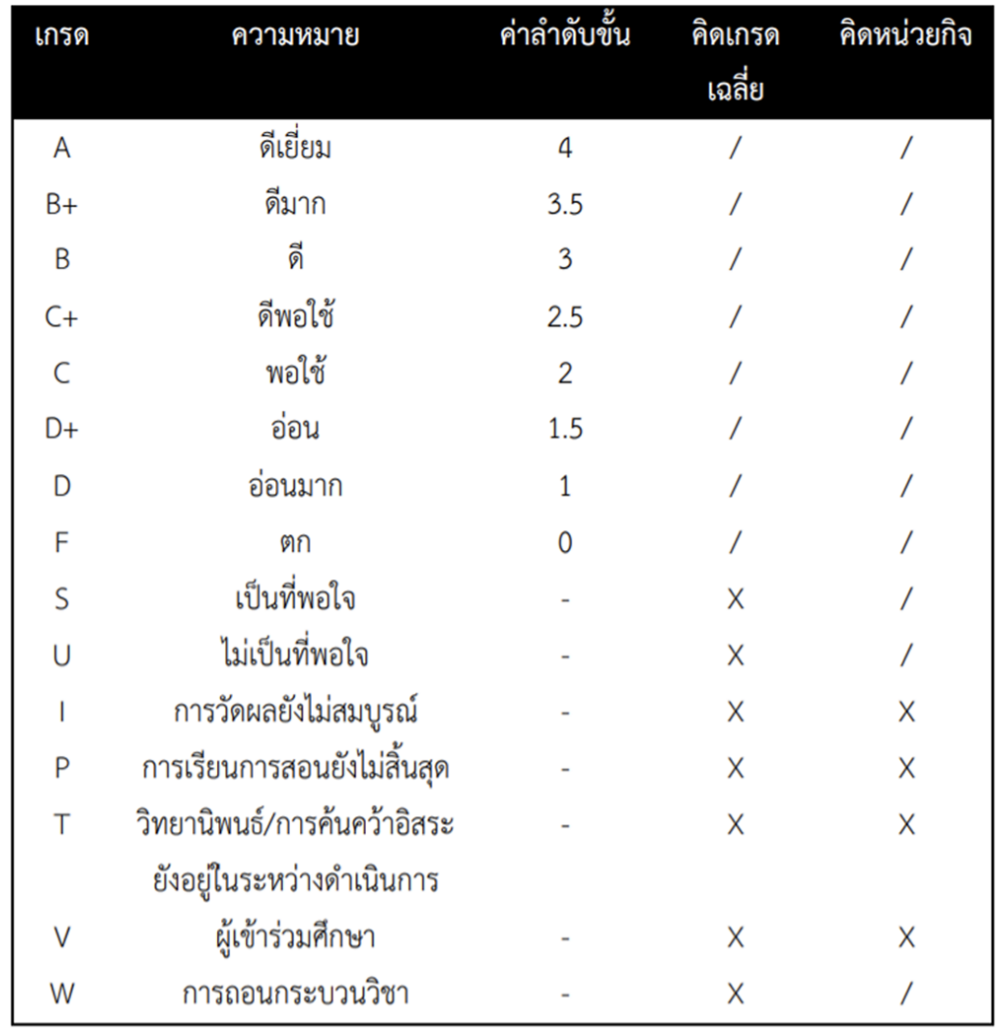
\includegraphics[width=0.8\textwidth]{all_grade.png}
    \caption{grade}
    \label{fig:grade}
  \end{center}
\end{figure}

% \begin{equation}\label{eq:dielectric}
%   k_1=\frac{\omega}{c({1/\varepsilon_m + 1/\varepsilon_i})^{1/2}}=k_2=\frac{\omega
%   \sin(\theta)\varepsilon_\mathit{air}^{1/2}}{c}
%   \end{equation}
% $$GPA=\frac{\sum_{i=1}^{\n}G_i\cdotP_i}{\sum_{i=1}^{\n}P_i}

\section{เกณฑ์มาตรฐานหลักสูตรระดับปริญญาตรี พ.ศ. 2558 ตามประกาศของกระทรวงศึกษาธิการ}
\subsection{โครงสร้างหลักสูตร}
ประกาศของกระทรวงศึกษาธิการฉบับนี้ได้กล่าวถึงโครงสร้างของหลักสูตรในระดับปริญญาตรีไว้ว่า โครงสร้าง
หลักสูตรต้องประกอบด้วยหมวดวิชาศึกษาทั่วไป หมวดวิชาเฉพาะ และหมวดวิชาเลือกเสรี โดยมีสัดส่วนจํานว
นหน่วยกิตของแต่ละหมวดวิชา ดังนี้
\begin{enumerate}
  \item  หมวดวิชาศึกษาทั่วไป หมายถึง หมวดวิชาที่เสริมสร้างความเป็นมนุษย์ที่สมบูรณ์ ให้มีความรอบรู้อย่าง
  กว้างขวาง เข้าใจ และเห็นคุณค่าของตนเอง ผู้อื่น สังคม ศิลปวัฒนธรรม และธรรมชาติ ใส่ใจต่อความ
  เปลี่ยนแปลงของสรรพสิ่ง พัฒนาตนเองอย่างต่อเนื่อง ดําเนินชีวิตอย่างมีคุณธรรม พร้อมให้ความช่วย
  เหลือเพื่อนมนุษย์ และเป็นพลเมืองที่มีคุณค่าของสังคมไทยและสังคมโลก
  สถาบันอุดมศึกษาอาจจัดวิชาศึกษาทั่วไปในลักษณะจําแนกเป็นรายวิชาหรือลักษณะบูรณาการใด ๆ
  ก็ได้ โดยผสมผสานเนื้อหาวิชาที่ครอบคลุมสาระของกลุ่มวิชาสังคมศาสตร์ มนุษยศาสตร์ ภาษาและ
  กลุ่มวิชาวิทยาศาสตร์กับคณิตศาสตร์ ในสัดส่วนที่เหมาะสม เพื่อให้บรรลุวัตถุประสงค์ของ หมวดวิชา
  ศึกษาทั่วไป โดยให้มีจํานวนหน่วยกิตรวมไม่น้อยกว่า 30 หน่วยกิต
  อนึ่ง การจัดวิชาศึกษาทั่วไปสําหรับหลักสูตรปริญญาตรี(ต่อเนื่อง) อาจได้รับการยกเว้นรายวิชาที่ได้
  ศึกษามาแล้วในระดับประกาศนียบัตรวิชาชีพชั้นสูงหรือระดับอนุปริญญา ทั้งนี้ จํานวนหน่วยกิตของ
  รายวิชาที่ได้รับการยกเว้นดังกล่าว เมื่อนับรวมกับรายวิชาที่จะศึกษาเพิ่มเติมในหลักสูตรปริญญาตรี
  (ต่อเนื่อง) ต้องไม่น้อยกว่า 30 หน่วยกิต
  \item หมวดวิชาเฉพาะ หมายถึง วิชาแกน วิชาเฉพาะด้าน วิชาพื้นฐานวิชาชีพและวิชาชีพ ที่มุ่งหมายให้ผู้
  เรียนมีความรู้ ความเข้าใจ และปฏิบัติงานได้ โดยให้มีจํานวนหน่วยกิตรวม ดังนี้
  \begin{itemize}
    \item หลักสูตรปริญญาตรี(4 ปี) ทางวิชาการ ให้มีจํานวนหน่วยกิตหมวดวิชาเฉพาะ รวมไม่น้อยกว่า
    72 หน่วยกิต
    \item หลักสูตรปริญญาตรี(4 ปี) ทางวิชาชีพหรือปฏิบัติการ ให้มีจํานวน หน่วยกิตหมวดวิชาเฉพาะ
    รวมไม่น้อยกว่า 72 หน่วยกิต โดยต้องเรียนวิชาทางปฏิบัติการตามที่ มาตรฐานวิชาชีพกําหนด
    หากไม่มีมาตรฐานวิชาชีพกําหนดต้องเรียนวิชาทางปฏิบัติการไม่น้อยกว่า 36 หน่วยกิต และ
    ทางทฤษฎีไม่น้อยกว่า 24 หน่วยกิต
    \item หลักสูตร (ต่อเนื่อง) ให้มีจํานวนหน่วยกิตหมวดวิชาเฉพาะรวมไม่น้อยกว่า 42 หน่วยกิต ในจํา
    นวนนั้นต้องเป็นวิชาทางทฤษฏีไม่น้อยกว่า 18 หน่วยกิต
    \item หลักสูตรปริญญาตรี(5 ปี) ให้มีจํานวนหน่วยกิตหมวดวิชาเฉพาะรวม ไม่น้อยกว่า 90 หน่วยกิต
    \item  หลักสูตรปริญญาตรี(ไม่น้อยกว่า 6 ปี) ให้มีจํานวนหน่วยกิตหมวดวิชา เฉพาะรวมไม่น้อยกว่า
    108 หน่วยกิต
 \end{itemize}
 สถาบันอุดมศึกษาอาจจัดหมวดวิชาเฉพาะในลักษณะวิชาเอกเดี่ยว วิชาเอกคู่ หรือวิชาเอกและวิชาโท
ก็ได้ โดยวิชาเอกต้องมีจํานวนหน่วยกิตไม่น้อยกว่า 30 หน่วยกิต และวิชาโทต้องมีจํานวนหน่วยกิตไม่
น้อยกว่า 15 หน่วยกิต ในกรณีที่จัดหลักสูตรแบบวิชาเอกคู่ต้องเพิ่ม จํานวนหน่วยกิตของวิชาเอกอีก
ไม่น้อยกว่า 30 หน่วยกิต และให้มีจํานวนหน่วยกิตรวมไม่น้อยกว่า 150 หน่วยกิต
สําหรับหลักสูตรปริญญาตรีแบบก้าวหน้า ผู้เรียนต้องเรียนวิชาระดับบัณฑิตศึกษาในหมวดวิชาเฉพาะ
ไม่น้อยกว่า 12 หน่วยกิต
\item  หมวดวิชาเลือกเสรี หมายถึง วิชาที่มุ่งให้ผู้เรียนมีความรู้ ความเข้าใจ ตามที่ ตนเองถนัดหรือสนใจ โดย
เปิดโอกาสให้ผู้เรียนเลือกเรียนรายวิชาใด ๆ ในหลักสูตรระดับปริญญาตรี โดยให้มีจํานวนหน่วยกิต
รวมไม่น้อยกว่า 6 หน่วยกิต สถาบันอุดมศึกษาอาจยกเว้นหรือเทียบโอนหน่วยกิตรายวิชาในหมวดวิชาศึกษาทั่วไป หมวดวิชาเฉพาะ
และหมวดวิชาเลือกเสรี ให้กับนักศึกษาที่มีความรู้ความสามารถ ที่สามารถวัดมาตรฐานได้ ทั้งนี้ นักศึกษาต้องศึกษาให้ครบตามจํานวนหน่วยกิตที่กําหนดไว้ในเกณฑ์มาตรฐานหลักสูตร และเป็นไป ตาม
หลักเกณฑ์การเทียบโอนผลการเรียนระดับปริญญาเข้าสู่การศึกษาในระบบ และแนวปฏิบัติที่ดี เกี่ยว
กับการเทียบโอน ของสํานักงานคณะกรรมการการอุดมศึกษา
\end{enumerate}
\subsection{เกณฑ์การวัดผลและการสําเร็จการศึกษา}
ให้สถาบันอุดมศึกษากําหนดเกณฑ์การวัดผล เกณฑ์ขั้นต่ําของแต่ละรายวิชา และเกณฑ์การสําเร็จการศึกษา
ตามหลักสูตร โดยต้องเรียนครบ ตามจํานวนหน่วยกิตที่กําหนดไว้ในหลักสูตร และต้องได้ระดับคะแนนเฉลี่ย
ไม่ตํ่ากว่า 2.00 จากระบบ 4 ระดับคะแนนหรือเทียบเท่า จึงถือว่าเรียนจบหลักสูตรปริญญาตรี
